% $Id: template.tex 11 2007-04-03 22:25:53Z jpeltier $

\documentclass{vgtc}                          % final (conference style)
% \documentclass[onecolumn]{vgtc}             % one column
%\documentclass[review]{vgtc}                 % review
%\documentclass[widereview]{vgtc}             % wide-spaced review
%\documentclass[preprint]{vgtc}               % preprint
%\documentclass[electronic]{vgtc}             % electronic version

% Make references appear in order of appearance
\bibliographystyle{unsrt}

% Add page numbers
\makeatletter
\renewcommand{\@oddfoot}{\hfil\thepage\hfil}
\renewcommand{\@evenfoot}{\@oddfoot}
\makeatother

%% Uncomment one of the lines above depending on where your paper is
%% in the conference process. ``review'' and ``widereview'' are for review
%% submission, ``preprint'' is for pre-publication, and the final version
%% doesn't use a specific qualifier. Further, ``electronic'' includes
%% hyperreferences for more convenient online viewing.

%% Please use one of the ``review'' options in combination with the
%% assigned online id (see below) ONLY if your paper uses a double blind
%% review process. Some conferences, like IEEE Vis and InfoVis, have NOT
%% in the past.

%% Figures should be in CMYK or Grey scale format, otherwise, colour 
%% shifting may occur during the printing process.

%% These few lines make a distinction between latex and pdflatex calls and they
%% bring in essential packages for graphics and font handling.
%% Note that due to the \DeclareGraphicsExtensions{} call it is no longer necessary
%% to provide the the path and extension of a graphics file:
%% \includegraphics{diamondrule} is completely sufficient.
%%
\ifpdf%                                % if we use pdflatex
  \pdfoutput=1\relax                   % create PDFs from pdfLaTeX
  \pdfcompresslevel=9                  % PDF Compression
  \pdfoptionpdfminorversion=7          % create PDF 1.7
  \ExecuteOptions{pdftex}
  \usepackage{graphicx}                % allow us to embed graphics files
  \DeclareGraphicsExtensions{.pdf,.png,.jpg,.jpeg} % for pdflatex we expect .pdf, .png, or .jpg files
\else%                                 % else we use pure latex
  \ExecuteOptions{dvips}
  \usepackage{graphicx}                % allow us to embed graphics files
  \DeclareGraphicsExtensions{.eps}     % for pure latex we expect eps files
\fi%

%% it is recomended to use ``\autoref{sec:bla}'' instead of ``Fig.~\ref{sec:bla}''
\graphicspath{{figures/}{pictures/}{images/}{./}} % where to search for the images

\usepackage{microtype}                 % use micro-typography (slightly more compact, better to read)
\PassOptionsToPackage{warn}{textcomp}  % to address font issues with \textrightarrow
\usepackage{textcomp}                  % use better special symbols
\usepackage{mathptmx}                  % use matching math font
\usepackage{times}                     % we use Times as the main font
\renewcommand*\ttdefault{txtt}         % a nicer typewriter font
\usepackage{cite}                      % needed to automatically sort the references
\usepackage{tabu}                      % only used for the table example
\usepackage{booktabs}                  % only used for the table example
%% We encourage the use of mathptmx for consistent usage of times font
%% throughout the proceedings. However, if you encounter conflicts
%% with other math-related packages, you may want to disable it.

\usepackage{makecell}
\usepackage{float}

%% If you are submitting a paper to a conference for review with a double
%% blind reviewing process, please replace the value ``0'' below with your
%% OnlineID. Otherwise, you may safely leave it at ``0''.
\onlineid{0}

%% declare the category of your paper, only shown in review mode
\vgtccategory{Research}

%% allow for this line if you want the electronic option to work properly
\vgtcinsertpkg

%% In preprint mode you may define your own headline.
%\preprinttext{To appear in an IEEE VGTC sponsored conference.}

%% Paper title.

\title{CityQuest - COMPSCI 732: Individual Report}

%% This is how authors are specified in the conference style

%% Author and Affiliation (single author).
%%\author{Roy G. Biv\thanks{e-mail: roy.g.biv@aol.com}}
%%\affiliation{\scriptsize Allied Widgets Research}

%% Author and Affiliation (multiple authors with single affiliations).
%%\author{Roy G. Biv\thanks{e-mail: roy.g.biv@aol.com} %
%%\and Ed Grimley\thanks{e-mail:ed.grimley@aol.com} %
%%\and Martha Stewart\thanks{e-mail:martha.stewart@marthastewart.com}}
%%\affiliation{\scriptsize Martha Stewart Enterprises \\ Microsoft Research}

%% Author and Affiliation (multiple authors with multiple affiliations)
\author{Romili Townsend \\ 
    \parbox{1.4in}{\scriptsize \centering University of Auckland}\\
    \parbox{1.4in}{\scriptsize \centering rtow454@aucklanduni.ac.nz}
}
%% Copyright space is enabled by default as required by guidelines.
%% It is disabled by the 'review' option or via the following command:
% \nocopyrightspace

%%%%%%%%%%%%%%%%%%%%%%%%%%%%%%%%%%%%%%%%%%%%%%%%%%%%%%%%%%%%%%%%
%%%%%%%%%%%%%%%%%%%%%% START OF THE PAPER %%%%%%%%%%%%%%%%%%%%%%
%%%%%%%%%%%%%%%%%%%%%%%%%%%%%%%%%%%%%%%%%%%%%%%%%%%%%%%%%%%%%%%%%

\begin{document}

%% The ``\maketitle'' command must be the first command after the
%% ``\begin{document}'' command. It prepares and prints the title block.

%% the only exception to this rule is the \firstsection command

\maketitle

%% \section{Introduction} %for journal use above \firstsection{..} instead
\section{Abstract}

CityQuest is a GPS-based mobile exploration game designed to encourage physical activity and improve users' familiarity with urban environments through navigation-based tasks.

The system assigns challenges at locations within the city that the user must travel to in order to complete. Gamification elements, such as streaks, levels, badges, and leaderboards are employed to make the system more motivating to users.

This report outlines the motivation, design, and implementation of this system developed for the COMPSCI 732 course, with a particular focus on methodology and tooling, and compares it to existing solutions. 

\section{Introduction: Introduce and motivate the project.} 

Tourists and new residents to a city often report difficulty with navigation {TODO: citation/data needed}. One key motive of this project is to aid these individuals in familiarising them with the area through gamified challenges which employ their navigation skills.

Additionally, a significant percent of the population do not meet daily exercise recommendations {TODO: citation needed}, and sedentary lifestyles are becoming increasingly common {TODO: citation needed}.

Existing research shows the effectiveness of gamification  in exercise {TODO: citation needed, what was found?}.

\section{Goals}

Create a GPS-based city exploration game that rewards movement and exploration of the local environment.

\begin{itemize}
    \item Encourage physical activity by rewarding users for walking and through fitness challenges.
    \item Improve users' familiarisation with their environment through interactions with local landmarks and points of interest.
    \item Provide an engaging, gamified alternative to traditional navigation tools.
\end{itemize}


\section{Related Work: What has been done before? Compare it with your project.}

Multiple existing exploration-based games exist. Notable examples include Pokemon Go and Ingress, both of which use GPS-backed movement tracking as a core gameplay mechanic.  

Google Maps is widely used navigation platform that supports users discovering nearby locations through features such as \textit{Search This Area}, which allows users to search within a geographic area for locations belonging to certain categories, such as restaurants or parks. Search results are curated based on proximity, user ratings, and popularity. In addition, Google Maps also provides comprehensive route planning with turn-by-turn instructions. 

While these features support location discovery and navigation, Google Maps is designed primarily to optimise travel efficiency through finding the fastest route to a location rather than encourage physical activity and exploration. In Google Maps, users select destinations and are guided to them, where CityQuest instead provides users with daily, location-backed challenges that encourage exploration, environmental interaction, and physical activity. In addition, CityQuest incorporates game mechanics to encourage exploration and movement, whereas Google Maps does not.

{TODO: compare it with my project}

\section{Design: Software architecture (e.g. class diagram)? User interface (e.g. screen diagram)? Why this design?}

We created an ERD with PlantUML during the initial system planning phase to visualise the relationships between entities within the system. As the system evolved, we updated this ERD to reflect the changes in the system. This final ERD can be see in Figure~\ref{fig:erd}. As can be seen in this ERD, there is an inherent relationship between each entity type in the database. 
For example, users are assigned user challenges, each of which corresponds to a challenge, and each of which which has an associated category. This highly relational nature of our database influenced our decision in choosing a relational database such as PostgreSQL over a document-oriented database such as MongoDB.

\begin{figure*}[t]
    \centering
    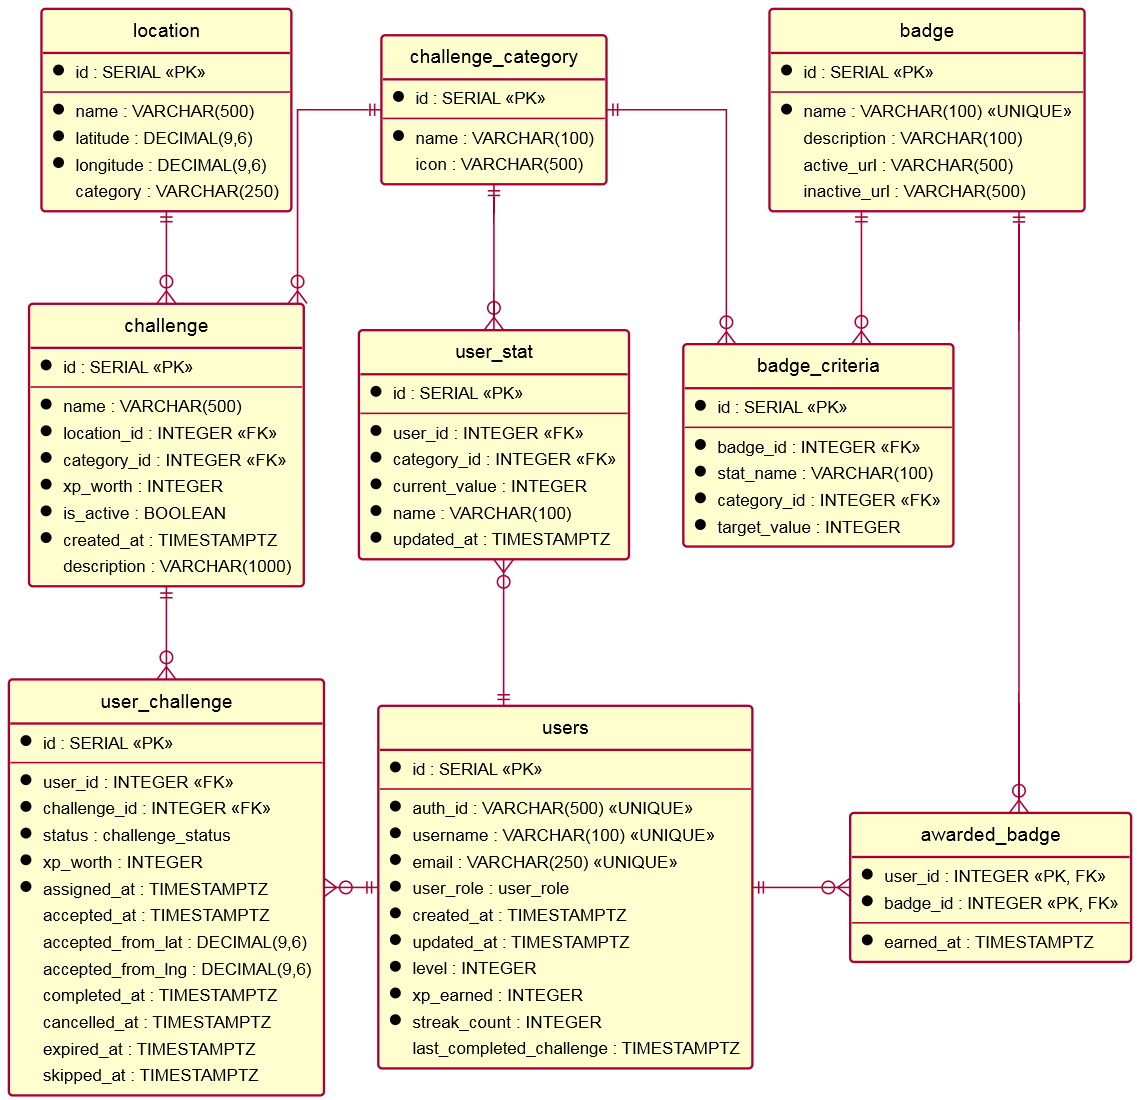
\includegraphics[width=0.7\linewidth]{erd.png}
    \caption{Entity Relationship Diagram of the CityQuest project}
    \label{fig:erd}
\end{figure*}

Our group created low-fidelity Figma mockups for the Challenge list, challenge map, achievements, and profile pages of the frontend system user interface, as can be see in Figures~\ref{fig:mockup-1} and~\ref{fig:mockup-2}. These prototypes were created to serve as inspiration for the in-development system, identify early and UX concerns, and ensure all group members had a consistent vision for the system.

\begin{figure}
    \centering
    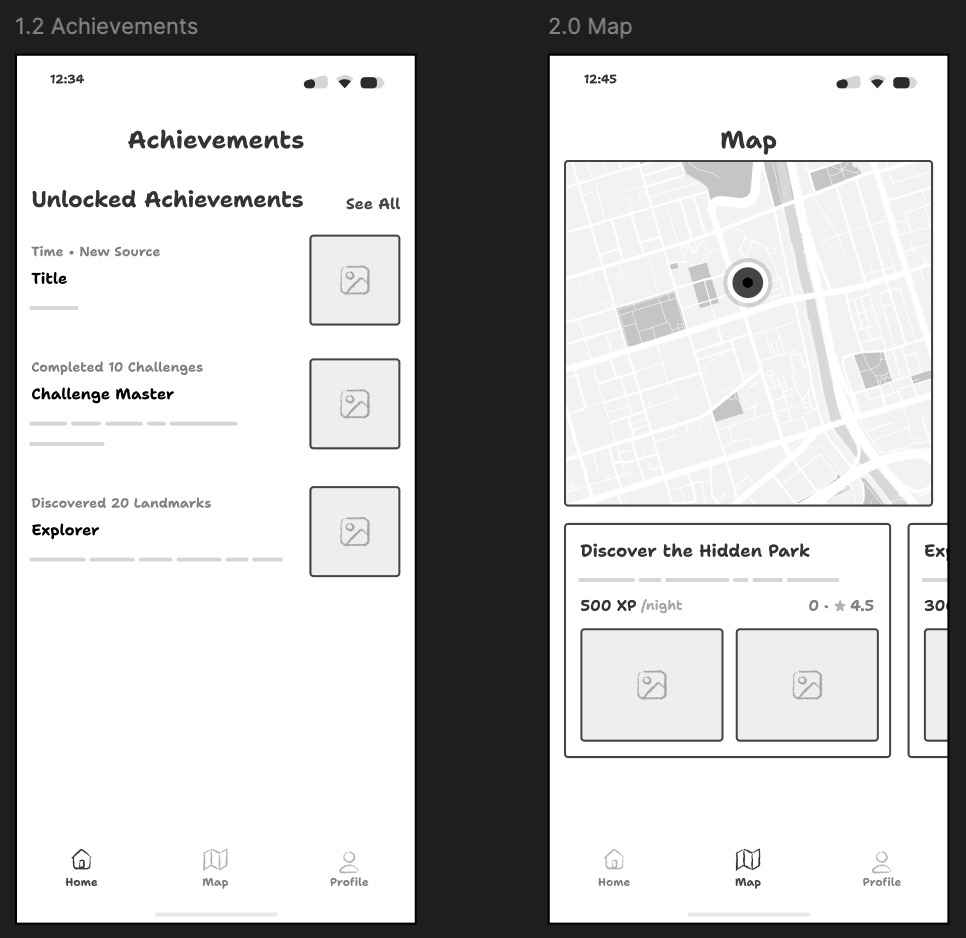
\includegraphics[width=0.9\linewidth]{Figma-1.png}
    \caption{Figma mockups of the Achievements and Map view pages}
    \label{fig:mockup-1}
\end{figure}

\begin{figure}
    \centering
    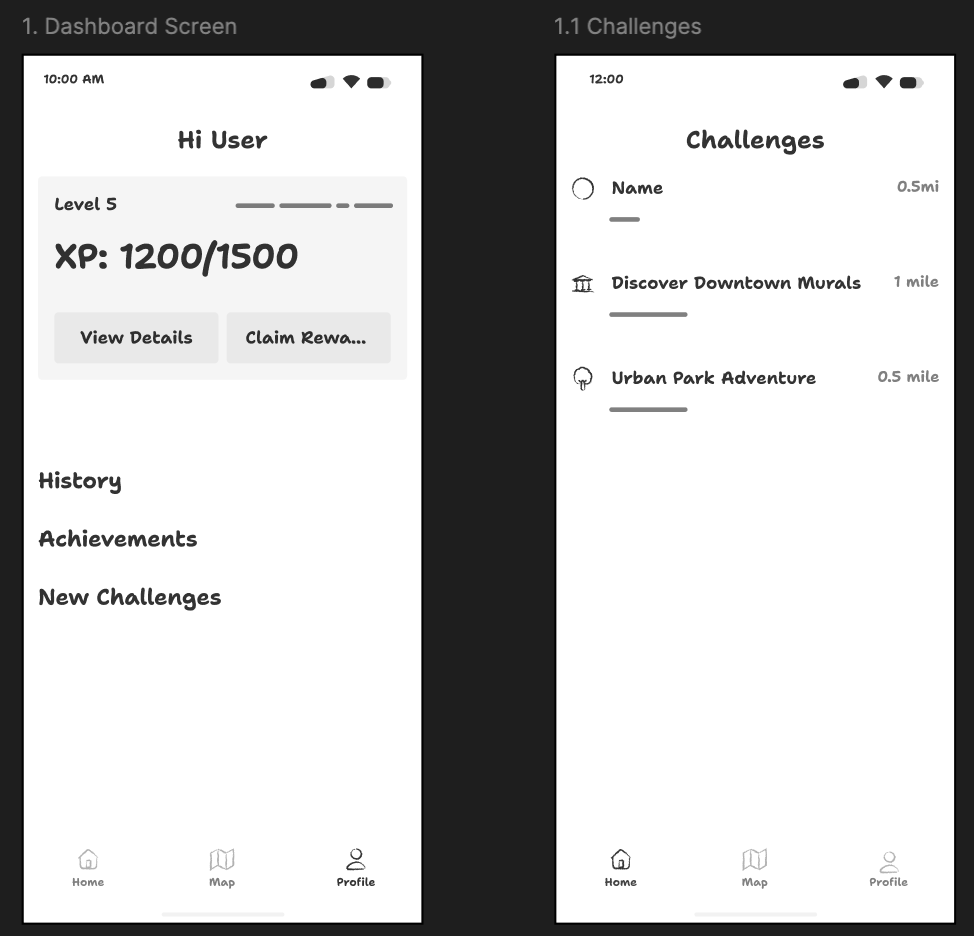
\includegraphics[width=0.9\linewidth]{Figma-2.png}
    \caption{Figma mockups of the Profile and Challenge view pages}
    \label{fig:mockup-2}
\end{figure}

\section{Implementation: What have you implemented?}

\section{Testing: How have you tested?}

Testing was done using Vitest and Playwright.
Unit tests were used to test individual functionalities.

The end-to-end tests were added to the GitHub Actions CI/CD pipeline to automatically trigger. On every commit to a branch, the testing suite runs and the outcome of these tests is displayed.

\section{Methodology: How has your team managed the project?}

Our team took part in weekly sprint meetings. During these meetings we took attendance and recorded all discussions as meeting minutes. This was done for future reference; if there is any uncertainty about what was discussed, team members can check the minute meetings to see what was discussed and what decisions were decided upon.
During the weekly sprints, we made a list of tasks to be completed this sprint and assigned each task to a person. To avoid ambiguity over whether a task's functionality has been fulfilled, for each task we clearly described what criteria would have to be met for that task to be marked as completed.

We used the MoSCoW method to prioritise tasks, grouping tasks by labels denoting their importance to the project, in order from most important to least important: Must haves, Should haves, Could haves, and Won't haves (out of scope).

{TODO: Mention PR reviews.}

For each task that we created, we added a corresponding issue ticket to GitHub. Commits referenced these issues so that team members can see what commits are responsible. Each pull request has a issue linked and was done in a suitable branch, so that viewing the commit history makes it clear which commits effect which issue.

\section{Tooling: What tools did you use to assist the development process (e.g. git, Jira, ChatGPT, etc...)? How effective were those tools? Any drawbacks (especially with the GenAI stuff)?}

Generative AI was used by some team members to increase efficiency, particularly for menial tasks where the code is easy to validate. 

Copilot code review was used in multiple instances to check for any bugs, syntax errors, and suggest considerations. However, this was not used as a substitute to human-run peer reviews but rather in addition to; all pull requests to the main branch were peer reviewed by at least one other team member.

\section{Discussion: Have the goals been achieved? Problems?}

A user study could be valuable to investigate whether this city exploration game had an impact on users' familiarity with their surroundings, and whether it increased users' physical activity levels, particularly average daily step counts. Unfortunately, due to the nature of the course, it was not feasible to conduct a user study.

In our project proposal we marked 13 tasks as must haves, 6 tasks as should haves, 10 tasks as could haves, and 4 tasks as out of scope.
Of these tasks, all must haves were completed, all should haves, 2 could haves, and no out of scope tasks.

The following table compares, for every prioritisation category, the number of tasks completed vs the number of tasks assigned.

\begin{table}[H]
    \centering
    \begin{tabular}{|c|c|c|c|}
        \hline
        Prioritisation & 
        \makecell{Completed\\tasks} & 
        \makecell{Assigned\\tasks} & 
        \makecell{Percent\\completed} \\
        \hline
        Must have & 13 & 13 & 100\% \\
        Should have & 6 & 6 & 100\% \\
        Could have & 2 & 10 & 20\% \\
        \hline
        Total (within scope)& 22 & 29 & 75.86\% \\
        \hline
        Won't have (outside scope)& 0 & 4 & 0\% \\
        \hline
    \end{tabular}
    \caption{Task completion summary by prioritisation category}
    \label{tab:completion_summary}
\end{table}

\section{Conclusion: Conclusions? Lessons learned? Reflections? Future work?}

%\bibliographystyle{abbrv}
\bibliographystyle{abbrv-doi}
%\bibliographystyle{abbrv-doi-narrow}
%\bibliographystyle{abbrv-doi-hyperref}
%\bibliographystyle{abbrv-doi-hyperref-narrow}

\bibliography{template}
\end{document}


